\documentclass[10pt,a4paper]{article}
\parindent=0cm
 
   \textheight 24cm
   \textwidth 16cm
\oddsidemargin=0cm

% \usepackage[french]{babel}
\usepackage[utf8]{inputenc}

\usepackage{graphicx}
\usepackage{caption}

\usepackage{url,amsmath,amssymb,amsthm,amsfonts,epsfig}
% eurosym,geometry}
% \selectlanguage{french}

\def\var{\mathrm{var}}
\def\BB{\mathcal{B}}
\def\FF{\mathcal{F}}
\def\Pa{\mathcal{P}}
\def\M{\mathcal{M}}
\def\P{\mathcal{P}}
\def\T{\mathcal{T}}
\def\L{\mathcal{L}}

\def\AA{\mathfrak{A}}
\def\S{\mathfrak{S}}
\def\SS{\mathcal{S}}
\def\CC{\mathcal{C}}

\def\A{\mathbb{A}}
\def\B{\mathbb{B}}
\def\D{\mathbb{D}}
\def\U{\mathbb{U}}


\def\bq{\begin{quote}\begin{em}}
\def\eq{\end{em}\end{quote}}

\def\un{\mathbf{1}}
\def\dd{\mathrm{d}}
\def\ee{\mathrm{e}}
\def\ii{\mathrm{i}}
\def\eps{\varepsilon}

\def\hth{\widehat{\theta}}
\def\ovx{\overline{X}}
\def\ima{\mathrm{Im}}

\newcommand{\C}{\mathbb C}
\newcommand{\R}{\mathbb R}
\newcommand{\N}{\mathbb N}
\newcommand{\Z}{\mathbb Z}
\newcommand{\Q}{\mathbb Q}

\newcommand{\espmes }{(\Omega, {\cal F})}
\newcommand{\espprob}{(\Omega, {\cal F}, P)}
\newcommand{\va}{variable al\'eatoire }
\newcommand{\vas}{variables al\'eatoires }
\newcommand{\Vas}{Variables al\'eatoires }
\newcommand{\cov}{\hbox{cov}}
\newtheorem{theo}{Théorème}[section]
\newtheorem{coro}{Corollaire}[section]
\newtheorem{lemm}{Lemme}[section]
\newtheorem{defi}[theo]{Définition}
\newtheorem{prop}[theo]{Proposition}
\newtheorem{rque}[theo]{Remarque}
\newtheorem{exem}[theo]{Exemple}
\newtheorem{exer}{Exercice}
\def\card{\mathrm{card}\,}

\newcommand{\tran}[1]{\,{}^{t}\!#1}
\renewcommand\det{\mathop{\textrm{d\'et}}}

\renewcommand{\le}{\leqslant}
\renewcommand{\ge}{\geqslant}
\def\demi{\frac{1}{2}}
\def\ds{\displaystyle}
\def\btheo{\begin{theo}}\def\etheo{\end{theo}}
\def\bcoro{\begin{coro}}\def\ecoro{\end{coro}}
\def\blemm{\begin{lemm}}\def\elemm{\end{lemm}}
\def\bdefi{\begin{defi}}\def\edefi{\end{defi}}
\def\bprop{\begin{prop}}\def\eprop{\end{prop}}
\def\brque{\begin{rque}}\def\erque{\end{rque}}
\def\bexem{\begin{exem}}\def\eexem{\end{exem}}

\def\bexer{\begin{exer}\begin{em}}\def\eexer{\end{em}\end{exer}}
\usepackage{graphics}
\usepackage{color}              % Need the color package
\usepackage{epsfig}
\def\F{{\cal F}}
\def\1{{\rm 1\kern-.8ex 1}}
\def\euro{\mbox{\raisebox{.25ex}{{\it =}}\hspace{-.5em}{\sf C}}} 
\newcommand{\bin}[2]{\left( \begin{array}{c} 
#1 \\#2\end{array}\right)}

\begin{document}
%\Large
\noindent Intro mod. num. 
\hfill Puissance \hfill {L3 \the\year}\\


\bexer
\textbf{Domaine de Gershgorin}

Soit $A\in {\cal M}_n(\C)$.
On note, pour $1\leq i\leq n$, $D_i$ la boule fermée dans $\C$ de 
centre $a_{i,i}$ et de rayon $\ds\sum_{j\not= i}|a_{i,j}|$.
Le domaine de Gershgorin, qu'on notera ${\cal G}(A)$ est la réunion des 
disques $D_i$ pour $1\leq i\leq n$.
Montrer que le spectre de $A$ est inclus dans ${\cal G}(A)$.

\eexer

\bexer \textbf{Stabilité}\\
Si $A$ est une matrice sym\'etrique, et si $\|(A-\lambda) u\| \leq
\varepsilon \| u\|$, montrer que la distance de $\lambda$ au spectre
de $A$ est inf\'erieure \`a $\varepsilon$ (on pourra utiliser une base
orthonormale de vecteurs propres de $A$).
\eexer


\bexer (Méthode de la puissance)\\ Soit
$A=\left(\begin{array}{ccc}99&1&0\\1&100&1\\0&1&98\end{array}\right)$.
\begin{enumerate} \item Montrer que $A$ est diagonalisable et en
	utilisant l'exercice sur le domaine de Gersggorin que ses
	valeurs propres appartiennent à $[97,102]$. \item
	Déterminer par la méthode de la puissance une approximation
	de la plus grande valeur propre de $A$.

Pour ceci, on écrira une fonction qui donnera une valeur approchée 
de la plus grande valeur propre, une valeur approchée d'un 
vecteur propre associé et le nombre d'itérations utilisées 
pour ce calcul. La fonction aura comme argument une matrice carrée, 
un nombre d'iterations maximales (pour un test d'arrêt) 
et epsilon mesurant une erreur maximale.

\item Expliquer pourquoi en appliquant la méthode de la puissance à $A-97I_3$, 
on accélere la convergence.


\item Que se passe t-il si on applique la méthode de la puissance à 
$A-\gamma I_3$ si $\gamma$ est la valeur trouvée à la question 2) ?
\end{enumerate}

\eexer


\bexer
(élimination)

Soit $A$ une matrice réelle de taille $n$.
On suppose que les valeurs propres de $A$ notées $\{\lambda_1,\ldots,\lambda_n\}$ sont deux à deux distinctes et vérifient :
\[|\lambda_1|<|\lambda_2|<\cdots <|\lambda_n|\]
On note $u_i$ un vecteur propre associé à $\lambda_i$, pour $1\leq i\leq n$.
\begin{enumerate}
 \item Montrer que $\{\lambda_1,\ldots,\lambda_n\}$ sont les valeurs 
propres de $\ ^tA$.
On note $v_i$ un vecteur propre de $\ ^tA$ associé à $\lambda_i$, pour $1\leq i\leq n$.
\item Montrer que si $i\not= j$, $\langle u_i,v_j\rangle =0$.
(On pourra calculer $\langle Au_i,v_j\rangle$ de deux manières).\\
Montrer que pour tout $1\leq i\leq n$, $\langle u_i,v_i\rangle\not=0$.

\item Soit $B=A-\lambda_n\frac{u_n\ ^tv_n}{\langle u_n,v_n\rangle}$.
Montrer que les valeurs propres de $B$ sont 
$\{0,\lambda_1,\ldots,\lambda_{n-1}\}$.

\item Donner une méthode utilisant la méthode de la puissance appliquée 
plusieurs fois pour trouver des valeurs approchées des valeurs propres 
de A et de ses vecteurs propres.

L'appliquer à la matrice de l'exercice précédent.
\end{enumerate}
\eexer


\bexer (valeurs propres conjuguées)

Si $A$ est une matrice réelle, sa plus grande valeur propre en module n'est
pas forcément réelle, $A$ peut avoir un couple de valeurs propres
complexes conjuguées de module maximal. On peut appliquer la
méthode de la puissance à un shift de $A$ dans le complexe, par
exemple $A-iI$, on peut aussi rester dans le réel en cherchant
une relation de récurrence approchée $u_{n+2}+au_{n+1}+bu_n$
(où $u_{n+1}=Au_n$ et $u_0$ aléatoire). Programmer les deux
méthodes et comparer l'efficacité avec une matrice aléatoire
réelle de taille 4 (non symétrique).

\eexer

\bexer
(itérations inverses)

Lorsqu'on a effectué quelques itérations de la méthode de la puissance,
on a une première approximation $\lambda$ 
de la valeur propre de module maximal.
Il peut alors être intéressant d'effectuer la méthode de la puissance
sur la matrice $(A-\lambda I)^{-1}$. Programmer cette méthode
et discuter les avantages (vitesse de convergence) et inconvénients
(précision du calcul de l'inverse). Testez sur l'une des matrices
de la feuille.

\eexer


\bexer

Utiliser la m\'ethode de la puissance pour d\'eterminer la norme
triple d'une matrice subordonn\'ee \`a la norme euclidienne.
\eexer

\bexer \textbf{PageRank}
Soit $P$ une matrice transpos\'ee d'une matrice stochastique,
c'est-\`a-dire une matrice carr\'ee de taille $N$ dont les coefficients v\'erifient
$$ a_{ij} \in [0,1], \quad \sum_{i=1}^N a_{ij} =1 $$
la somme des coefficients d'une colonne donn\'ee vaut 1.\\
L'algorithme PageRank de Google construit une telle matrice \`a partir
du graphe connectant les pages web entre elles en posant
$a_{ij}=\frac{1}{n_j}$ si la page $j$ pointe vers la page $i$ et 0
sinon, avec $n_j$ le nombre de liens \'emis par la page $j$ (chaque lien
repr\'esente en quelque sorte un vote, dont le poids est pond\'er\'e
par le nombre de liens). 

On considère
le
reseau :

\begin{figure}[ht]
\begin{center}
	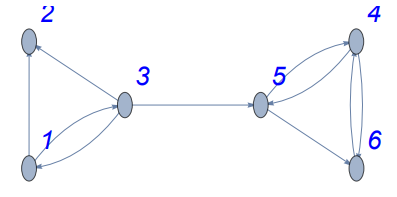
\includegraphics[scale=.4]{./graph1.png}
\end{center}
\end{figure}

dont la matrice d'adjacence (de connectivité) $C$ est

% https://perso.liris.cnrs.fr/pierre-edouard.portier/teaching_2014_2015/ia/pr/pr.pdf

\begin{figure}[ht]
\begin{center}
	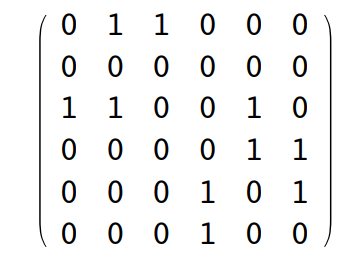
\includegraphics[scale=.4]{./adj_matrix.png}
\end{center}
\end{figure}

\begin{enumerate}
	\item Dessiner le graphe  dont la matrice d'adjacence $C$
		est $C^2$.
	\item Trouver les valeurs propres de $C$ avec
		\textbf{numpy}
	\item Pourquoi $0$ est valeur propre ? 
	\item Calculer la matrice $\tilde{C}$ (voir le cours).
	La  matrice est stochastique ?

	
\end{enumerate}


L’idée de Brin et Page pour permettre la découverte d’une
distribution stable par multiplication itérée de la matrice
stochastique est d’introduire la métaphore du “surfeur aléatoire” (random surfer). Cette métaphore permet en fait de
rendre la matrice ergodique. Le surfeur suit la structure
des liens du web, sauf que de temps en temps il décide
d’entrer une URL dans la barre de navigation afin de
sauter vers une page quelconque non nécessairement
connectée à la page courante. On appelle cette opération
la téléportation. La téléportation est aléatoire : chaque
page est équiprobable en tant que destination d’une opération de téléportation. On fait une combinaison convexe de
$C$ et de la matrice qui représente l’opération de
téléportation.

\begin{enumerate}
	\item Rendre $\tilde{C}$ stochastique comme expliquer dans
		le cours: $$ \alpha E + (1-\alpha)\frac{1}{n}
		e.e^T.$$
	\item Utiliser la méthode de  la puissance pour calculer la
		plus grande valeur propre.
	\item Trouver le vecteur propre associé. Donner une
		interpretation du vecteur propre.

\end{enumerate}
\eexer

\bexer
{\bf Méthode $QR$ pour le calcul de valeurs propres}\\

Soit une matrice $A\in\mathcal{M}_n(\mathbb{R})$ inversible. Dans cet exercice, on va utiliser la décomposition $QR$ pour déterminer toutes les valeurs propres de $A$. Pour cela, on définit une suite de matrices de la manière suivante : \\

$A_1 =  A$, puis pour tout $k\geq1$,

$$\left\{
\begin{aligned}
& (Q_k, R_k) =  \hbox{décomposition QR de } A_k\\
&A_{k+1} = R_k Q_k
\end{aligned}
\right.$$ 

\begin{itemize}

\item Montrer que les matrices $A_k$ construites au cours des itérations sont toutes semblables à $A$. Elles ont donc les mêmes valeurs propres que $A$. 

\item On suppose que les valeurs propres de $A$ sont toutes de
	modules différents ($|\lambda_1|>\cdots>|\lambda_n|$). Soit
	$P\in\mathrm{GL}_n(\mathbb{R})$ telle que $P^{-1}AP=diag(\lambda_1,\cdots,\lambda_n):=\Lambda$. On suppose que $P^{-1}$ admet une factorisation $LU$. Montrer qu'alors

$$\lim_{k\rightarrow +\infty} (A_k)_{ii} =\lambda_i,\hspace{0.3cm}\forall \  i,\hspace{1cm}\hbox{et}\hspace{1cm} \lim_{k\rightarrow +\infty} (A_k)_{ij} = 0,\hspace{0.3cm}\forall \ 1\leq j<i \leq n.$$

\item Implémenter cette méthode et vérifier numériquement que la vitesse de convergence dépend de $\max_i \ | \frac{\lambda_{i+1}}{\lambda_i} |$.

\item
Trouver des valeurs approchées 
des valeurs propres de 
 \[A=\left(\begin{array}{ccccc}
0&1&0&0&0\\1&1&1&0&0\\0&1&1&1&0\\0&0&1&1&1\\0&0&0&1&2
\end{array}\right)\]
Observer la forme des matrices intermédiaires.

% Pour une matrice g\'en\'erale, on utilise la forme de Hessenberg avant
% de faire la m\'ethode QR.

\end{itemize}

\eexer


\end{document}

\bexer

On consid\`ere l'\'equation diff\'erentielle 
$$ -u'{'}+\alpha u=f, \quad x \in [0,1], \quad u(0)=u(1)=0 $$
\begin{enumerate}
\item Discuter en fonction de $\alpha$ le nombre de solutions pour
  $f=0$. Comparer les conditions aux bords
avec le cas des conditions initiales $u(0)=0, u'(0)=0$.
\item On pose $\alpha>0$.
 D\'eterminer $a$ et $l$ de la formulation ``faible'' de cette \'equation
$ a(u,v)=l(v)$ pour tout $v$ de classe $C^1$ par morceaux nulle aux
bords.
\item Montrer que $a$ est sym\'etrique d\'efinie positive.
\item V\'erifier que la solution de $a(u,v)=l(v)$ est un extr\^emum
de  $J(u)=\frac12 a(u,u)-l(u)$ (formulation variationnelle de
l'\'equation diff\'erentielle).
\item Soit $N\geq2$, $h=1/N$ et $x_k=kh=k/N$ pour $k=0,..N$.\\
Pour $1\leq k \leq N-1$, on 
note $\phi_k(x)=\mbox{max}(0,1-|(x-x_k)/h|)$ la fonction 
atteignant son maximum 1 en $x_k$ et de
pente $\pm 1/h$ entre $[x_{k-1},x_{k+1}]$.\\
On va chercher le minimum de $J$ sur l'espace vectoriel
$E$ de dimension finie engendr\'e par les fonctions $\phi_k$
(c'est la projection orthogonale par rapport au produit scalaire 
induit par $a$ de la solution sur $E$, pourquoi~?)
D\'eterminer $a_{j,k}=a(\phi_j,\phi_k)$, $l_k=l(\phi_k)$.
\item Montrer que le minimum $u$ de $J$ sur $E$ v\'erifie $a(u,v)=l(v)$ pour
tout $v \in E$. En d\'eduire une matrice $A$ telle que
$A(u(x_j))_{j=1..N-1}=(l_j)_{j=1..N-1}$.
\item D\'eterminer $u(x_j)$ puis $u$.
\item Tracer sur une m\^eme figure $u$ et la solution exacte
pour $f(t)=1$ et pour $f(t)=t(1-t)$ pour $N=3$ et $N=10$.
\item Pour $N$ grand, quel est le cout de l'\'etape matricielle de la r\'esolution
par le pivot de Gauss~? Comparer avec la m\'ethode de Jacobi.
\item Que faut-il modifier lorsque $\alpha$ d\'epend de $x$~?
Comment se compare cette m\'ethode avec la m\'ethode des diff\'erences
finies de la feuille 1~?
\end{enumerate}

\eexer

\bexer
Soit $P$ un polyn\^ome unitaire de degr\'e $d>0$ \`a coefficients
r\'eels 
(ou complexes)
$$ P=x^d+p_{d-1}x^{d-1}+...+p_1x+p_0$$
On suppose que $P$ admet une seule racine de
module maximal, que l'on notera $z$. 
On souhaite trouver une approximation de $z$
par une m\'ethode combinant la m\'ethode de la puissance et de Newton.
Par exemple pour fixer les id\'ees et tester~:
$$ P=x^7-11x^4+5x-55, \quad d=7$$
\begin{enumerate}
\item On construit une matrice compagnon $M$ de $P$ (commande
\verb|M:=tran(companion(P))| de Xcas) d\'efinie par~:
$$ M=\left(\begin{array}{cccccc}
0 & 1 & 0 & ... & 0 & 0 \\
0 & 0 & 1 & ... & 0 & 0 \\
...& ... & ... & ... & ... & ... \\
0 & 0 & 0 & ... & 1 & 0 \\
0 & 0 & 0 & ... & 0 & 1 \\
-p_0 & -p_1 & -p_2 & ... & -p_{d-2} & -p_{d-1} \\
\end{array}\right)$$
on admettra que le polyn\^ome caract\'eristique
de $M$ est $P$. Expliquer pourquoi la m\'ethode de la puissance
appliqu\'ee \`a $M$ permet de d\'eterminer la racine $z$ de $P$.
\item En utilisant la structure particuli\`ere
de la matrice $M$, expliquer comment on peut calculer 
efficacement $v_{n+1}=Mv_n$ \`a partir de la liste $l$
des coefficients de $P$ par ordre croissant 
(\verb|l:=revlist(symb2poly(P,x))|) 
en $O(d)$ op\'erations.
\item \'Etant donn\'e un petit r\'eel $\varepsilon>0$, 
quel test d'arr\^et vous parait le plus judicieux pour
stopper le calcul des $v_n$~? Pourra-t-on certifier que l'estimation
de la valeur propre obtenue sera proche \`a $\varepsilon$ pr\`es de $z$~?
\item Programmer l'algorithme en passant en param\`etre
la liste \verb|l| et le petit r\'eel \verb|eps|
(on pourra utiliser \verb|v[1..d-1]|
qui extrait les \'el\'ements de \verb|v| d'indice \verb|1| \`a \verb|d-1|
inclus, \verb|dotprod(l,v)|
effectue le produit scalaire de \verb|l| et \verb|v| en tronquant
le vecteur le plus long lorsqu'ils ne sont pas de taille \'egale, 
et les instructions \verb|append| et \verb|normalize|)
\item Dans les questions suivantes, sauf la derni\`ere, on travaille
sur l'exemple. Donner une estimation $z_4$ de $z$
pour l'exemple pour $\varepsilon$=\verb|1e-4| et $z_8$ pour
$\varepsilon$=\verb|1e-8|. Combien d'it\'erations sont-elles
n\'ecessaires pour obtenir cette estimation~?
Pouvait-on s'y attendre~?
\item Afin d'acc\'el\'erer le calcul, on se propose d'utiliser la suite
it\'erative $u_n$ de la  m\'ethode de Newton en partant de $u_0=z_4$.
Donner l'expression de $u_{n+1}$ en fonction de $u_n$.
Quelle pr\'ecision peut-on esp\'erer 
en effectuant 2 it\'erations~?
\item Calculer $u_2$. Proposer un raisonnement pour
majorer l'erreur $|u_2-z|$ et calculer ce majorant.
\item Si on souhaite g\'en\'eraliser la m\'ethode ci-dessus \`a un
polyn\^ome unitaire quelconque (sans faire l'hypoth\`ese de
l'existence d'une unique racine de module maximal), quels
sont les obstacles pr\'evisibles~? Comment peut-on les contourner~?
\end{enumerate}

\eexer 

\end{document}
